\documentclass[11pt, notitlepage, leqno]{article}

%package imports
\usepackage[T1]{fontenc}
\usepackage[letterpaper, margin=1in]{geometry}  %for letter-sized paper
\usepackage{setspace}              %double spacing
\usepackage{fancyhdr}              %header capability
\usepackage{graphicx}
\usepackage{booktabs}
\usepackage{amsmath}
\usepackage{amssymb}
\usepackage{amsthm}
\usepackage{wrapfig}
\usepackage{tikz}
\usetikzlibrary{automata,positioning,arrows}
\usepackage{textcomp}

%page layout setup
\setlength{\headheight}{14.5pt}
\setlength{\headsep}{25pt}

%header setup
\pagestyle{fancyplain}
\fancyhf{}

\lhead{\fancyplain{}{\today}}                 %top left
\chead{\fancyplain{}{CPSC 121: Assignment 4}}                                 %top center
\rhead{\fancyplain{}{Calvin Cheng \& Brian Wu}}	                    %top right
\lfoot{\fancyplain{}{}}                                 %bottom left
\cfoot{\fancyplain{}{---\thepage---}}                   %bottom center
\rfoot{\fancyplain{}{}}                                 %bottom right

\renewcommand{\headrulewidth}{0pt}
\renewcommand{\footrulewidth}{0pt}

\renewcommand{\qedsymbol}{$\blacksquare$}

\newcommand{\unit}[1]{\;\textrm{#1}}
\renewcommand{\neg}{\mathord{\sim}}

\newcommand*\adjustwrapfigitem{\null\vskip-\baselineskip}

%document beginning
\begin{document}

%line spacing
\setstretch{1.0}

\begin{enumerate}

\item \begin{enumerate}

\item $\forall n \in \mathbb{Z}^{+}, \textrm{Odd}(n) \to \exists i \in \mathbb{Z}^{+}, \exists j \in \mathbb{Z}^{+}, n = i^2 - j^2$

\item \begin{proof}
Without loss of generality, let $n$ be an arbitrary unspecified positive integer. Assume that $n$ is odd, so that $n = 2k + 1$ for some $k \in \mathbb{N}$. Therefore,
\begin{align*}
	2k+1 &= 1(2k+1) \\
	&= (1 + k - k) (2k + 1) \\
	&= ((k+1) - k) ((k + 1) + k)\\
	&= (k+1)^2 - k^2
\end{align*}
As shown, every odd positive integer can be represented as the difference of two consecutive perfect squares.
\end{proof}
\end{enumerate}

\item \begin{enumerate}

\item $\forall a \in \mathbb{Z}, \forall b \in \mathbb{Z}, \forall c \in \mathbb{Z}, \neg(a \mid (b-c)) \to \neg(a \mid b) \vee  \neg(a \mid c)$

\item \begin{proof}
Without loss of generality, let $a$, $b$, and $c$ represent any arbitrary integers, so that $\neg(a \mid (b-c)) \to \neg((a \mid b) \wedge (a \mid c))$, by applying De Morgan's Law to the original statement. Thus, by the method of proof by contrapositive, let us assume that $a$ divides $b$ and that $a$ divides $c$, such that $b=aj$ and $c=ak$ for some integers $j$ and $k$. Then,
\begin{align*}
b - c  &= aj - ak\\
&= a(j-k)
\end{align*}
Therefore, because $j-k$ is an integer, $a$ must divide $b-c$, completing the proof of the contrapositive of the original statement.
\end{proof}

\end{enumerate}

\item \begin{proof}Without loss of generality, let $n$ be an unspecified arbitrary integer. Assume that $n$ is greater than 3.

First, let $m$ be an unspecified arbitrary integer. Assume that $(2 \mid m)$ and $(3 \mid m)$, so $\frac{m}{2}$ and $\frac{m}{3}$ are both integers. Therefore, their difference must be an integer as well:
\begin{align}
	\frac{m}{2} - \frac{m}{3} = \frac{3m}{6} - \frac{2m}{6} = \frac{m}{6} \in \mathbb{Z}
\end{align}
As a result, for any integer $m$ where $\frac{m}{2}$ and $\frac{m}{3}$ are both integers, $\frac{m}{6}$ must be an integer as well.

Secondly, let $a$ be an arbitrary even integer such that $a=2k$ for some integer $k$, and let $b$ be any arbitrary integer. Their product, then, must be an even integer as well, as shown:
\begin{align}
	&a \times b = 2kb = 2(kb)\notag\\
	&\therefore (2 \mid ab)
\end{align}

Since at least one integer of the three consecutive integers $n$, $n-1$, and $n-2$ must be even, $n(n-1)(n-2)$ must be even and divisible by 2, from the conclusion of (2).

Since one of the three consecutive integers must be divisible by 3, $n(n-1)(n-2)$ must be divisible by 3 as well, because the product of these three numbers will simply be a multiple of the integer that is divisible by three, whether it be $n$, $n-1$, or $n-2$.

Therefore, from the conclusion of (1), $\frac{n(n-1)(n-2)}{6}$ must be an integer for all $n \geq 3$, seeing as $\frac{n(n-1)(n-2)}{2}$ and $\frac{n(n-1)(n-2)}{3}$ are both integers.
\end{proof}

\item \begin{proof} Suppose the opposite is true. That is, assume that every student has talked to at least one other student, and that no two students talked to exactly the same number of people.

Let $N$ represent the size of the group of students. Then, let us start by assuming that one student talked to one other student only. The next student, then, must have talked to at least two other students, as one of the premises states that no two students talked to the same number of people. Let us assume that this student only talked to two other students.

The third student, then, must have talked to at least three students by the same logic as above, and this pattern continues on until the $N$th student is reached. Based on the established intuition, it is expected that the $N$th student talked to at least $N$ other students. However, given that students do not talk to themselves, this is impossible, because the maximum number of students that a student can talk to is $N-1$ (everyone but him/herself). Our original assumption thus leads to a contradiction, and therefore it must be true that if every student has talked to at least one other student, then two of the students talked to exactly the same number of people.
\end{proof}

\item \begin{enumerate}

\item A DFA for the problem is shown below:

\begin{tikzpicture}[>=stealth',shorten >=1pt,auto,node distance=2cm] 
	\node[state,initial] (s0)   {0\textcent}; 
	\node[state] (s1) [above right=of s0] {10\textcent};
	\node[state] (s2) [right=of s1] {20\textcent}; 
	\node[state] (s3) [below right=of s2] {30\textcent}; 
	\node[state] (s4) [below right=of s0] {25\textcent}; 
	\node[state,accepting](s5) [right=of s4] {35\textcent+};
	\path[->] 
	(s0) edge node {10} (s1)
	edge node [swap] {25} (s4)
	(s1) edge node {10} (s2)
	edge [bend left=10] node {25} (s5)
	(s2) edge node {10} (s3)
	edge node {25} (s5)
	(s3) edge node {10, 25} (s5)
	(s4) edge [bend left=10] node {10, 25}(s5)
	(s5) edge [bend left=10] node {10} (s1)
	edge [bend left=10] node {25} (s4);
\end{tikzpicture}

\item A circuit that implements the DFA above is shown below. State 0 represents 0\textcent\ inserted, 1 represents 10\textcent\ inserted, 2 represents 20\textcent\ inserted, 3 represents 25\textcent\ inserted, 4 represents 30\textcent\ inserted, and 5 represents 35\textcent\ or more inserted. Input 0 denotes the insertion of a dime, and Input 1 denotes the insertion of a quarter.
\begin{center}
\includegraphics[scale=0.096]{Circuit}
\end{center}

\end{enumerate}

\end{enumerate}

\end{document}